% Chapter 5

\chapter{Time Series} % Main chapter title

\label{Chapter5} % For referencing the chapter elsewhere, use \ref{Chapter5} 

\lhead{Chapter 5. \emph{Time Series}} % This is for the header on each page - perhaps a shortened title

%----------------------------------------------------------------------------------------

This chapter will explore the use of time series analysis techniques to generate models for forecasting prices in various national stock market indices. Usually, in trying to predict the future behaviour of financial markets the direction they will move, either up or down, is of more interest than the actual value itself. Thus, in this chapter predictions of the future direction as well as the actual value itself are attempted.  A variety of time series models are developed using exponential smoothing, ARIMA and hybrid ARIMA methods.

\section{Exponential Smoothing}

Exponential smoothing was applied to the stock market indice data sets in order to generate predictions for the following day's closing price, so-called one step ahead forecasts. Two basic approaches and an exponential smoothing methodology were examined. The two basic methods provide a useful baseline against which to compare later models, and are the mean and drift methodologies. The mean is simply the average of the data points in the sample while the drift is equivalent to drawing a straight line between the first and last point of the sample and then extrapolating this line forward the desired number of observations.

\subsection{Base Time Series Models}
Figure \ref{fig:chp5_ts_dax} shows the two base methods, mean and drift, being applied to a data set derived from the German Dax. The models were trained on the first 3000 observations of the Dax data set and tested on the remaining ones. The actual data points being predicted in Figure \ref{fig:chp5_ts_dax} are added to the plot in Figure \ref{fig:chp_ts_dax_act}. A variety of error measures for the two methods are listed in Table \ref{tab:chp_ts:sma}. From these error measures we can see that the drift model fits the training data the best, having the smallest error values across all the measures, but that the mean model actually performs the best on the test data.

%label - tab:chp_ts:sma
% latex table generated in R 3.1.0 by xtable 1.7-3 package
% Tue May 27 13:22:33 2014
\begin{table}[ht]
\centering
\caption[Simple forecasting methods.]{Mean, Naive and Drift methods applied to 
         to the Dax.} 
\label{tab:chp_ts:sma}
\begin{tabular}{llcccc}
  \toprule  & RMSE & MAE & MPE & MAPE & MASE \\ 
  \midrule Mean Training Set & 1394 & 1183 & -8 & 25 & 1 \\ 
  Mean Test Set & 208 & 163 & 2 & 3 & 3 \\ 
  Naive Training Set & 84 & 61 & -0 & 1 & 0 \\ 
  Naive Test Set & 303 & 263 & -5 & 5 & 4 \\ 
  Drift Training Set & 84 & 61 & -0 & 1 & 0 \\ 
  Drift Test Set & 302 & 262 & -5 & 5 & 4 \\ 
   \bottomrule \end{tabular}
\end{table}


\begin{figure}[tbh]
\centering
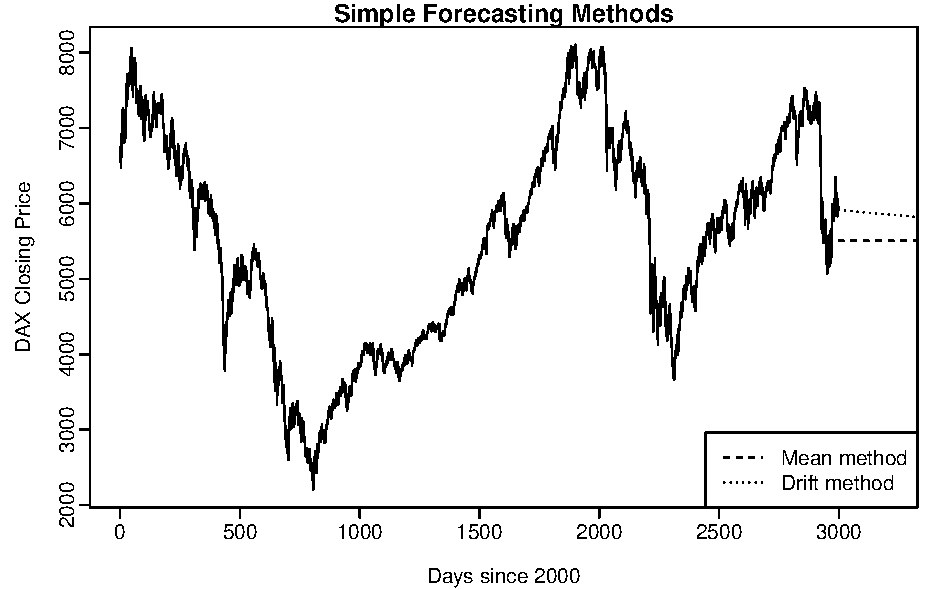
\includegraphics{Figures/chp_ts_dax1}
\caption[Forecasts generated by mean and drift methods]{Forecasts generated by mean and drift methods.}
\label{fig:chp5_ts_dax}
\end{figure}

\begin{figure}[tbh]
\centering
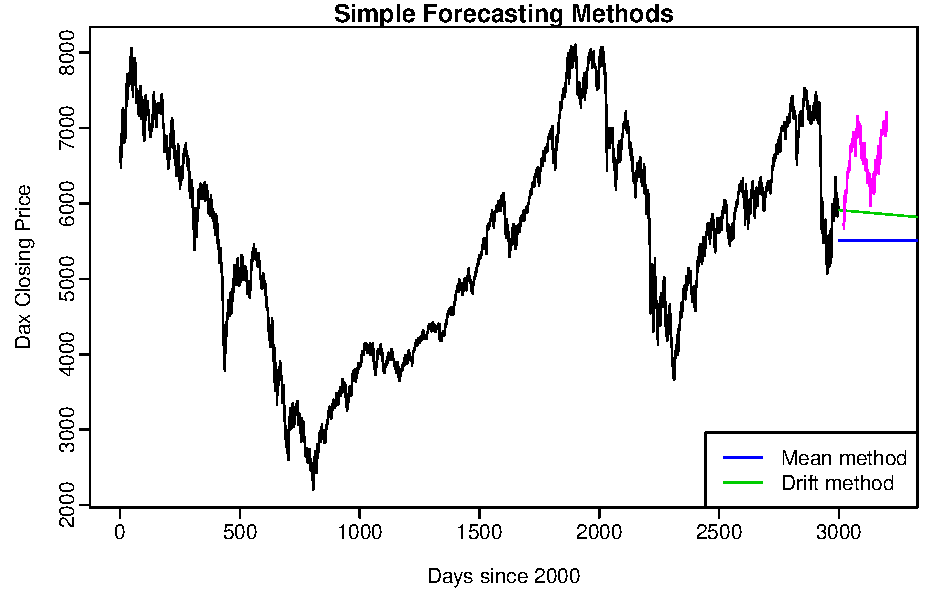
\includegraphics{Figures/chp_ts_dax1_plus_act_data}
\caption[Forecasts generated by mean and drift methods and actual data]{Forecasts generated by mean and drift methods with actual data in forecast period added.}
\label{fig:chp_ts_dax_act}
\end{figure}

Looking at Figure \ref{fig:chp_ts_dax_act} it can be seen that neither the mean or the drift does a good job with the predictions for the Dax. The forecasts were based on the entire data set, treating it as a homogeneous whole. However, financial time series typically shows a variety of behaviour at different periods. On occasions it is stationary and at other times trending. Thus, in the following sections, in order to generate forecasts a sliding window approach was adopted. A window of data (the last 30 observations) was used to generate a model and the one step ahead forecast, before the window was advanced one observation to the next period. In this way the model is constantly adapting and changing. Using this approach forecasts and models for use in a trading system from a mean, drift and exponential smoothing methodology were developed.

\subsection{Trading System Based on Mean Model}
\label{sec:es:mean}
Results from a trading system using the one step ahead forecasts generated by the mean model using a moving window can be seen in Table \ref{tab:es_mean_sys}. A trading algorithm, which can be seen in Appendix \ref{AppendixA} section \ref{appA:es_1}, used these forecasts to decide in which direction to trade. If the forecast was higher than the closing price a long trade was entered the following day and likewise if it was below the close a short trade was entered.


%label - tab:es_mean_sys
% latex table generated in R 3.1.0 by xtable 1.7-3 package
% Mon Jul 07 20:34:26 2014
\begin{table}[ht]
\centering
\caption[Results from the mean base ES System]{Results from the mean base ES System.} 
\label{tab:es_mean_sys}
\begin{tabular}{lcccccc}
  \toprule Mkt & LongPL & ShortPL & L Win \% & Av L PL & S Win \% & Av S PL \\ 
  \midrule Dax & -1640 & -1505 & 50 & -1 & 45 & -1 \\ 
  CAC & -1086 & 3553 & 52 & -1 & 51 & 2 \\ 
  FTSE & 1680 & 345 & 53 & 1 & 49 & 0 \\ 
  Dow & 8356 & -2126 & 54 & 7 & 46 & -1 \\ 
  Nikkei & -32 & 10646 & 51 & 0 & 53 & 6 \\ 
  AORD & -1333 & -2149 & 50 & -1 & 46 & -1 \\ 
   \bottomrule \end{tabular}
\end{table}


\subsection{Trading System Based on Drift Model}
In a similar way to the mean model of section \ref{sec:es:mean} the predictions generated by the drift model were passed the trading algorithm and the results can be seen in Table \ref{tab:es_drift_sys}. 

%label - tab:es_drift_sys
% latex table generated in R 3.1.0 by xtable 1.7-3 package
% Thu Jul 10 20:50:38 2014
\begin{table}[ht]
\centering
\caption[Results from the drift base ES System]{Results from the drift base ES System.} 
\label{tab:es_drift_sys}
\begin{tabular}{lcccccc}
  \toprule Mkt & LongPL & ShortPL & L Win \% & Av L PL & S Win \% & Av S PL \\ 
  \midrule Dax & 2310 & 2445 & 54 & 1 & 50 & 2 \\ 
  CAC & -2422 & 2217 & 49 & -1 & 48 & 2 \\ 
  FTSE & -518 & -1853 & 51 & 0 & 47 & -1 \\ 
  Dow & 5416 & -5066 & 54 & 3 & 46 & -4 \\ 
  Nikkei & -6939 & 3739 & 48 & -4 & 50 & 3 \\ 
  AORD & 1476 & 660 & 53 & 1 & 49 & 1 \\ 
   \bottomrule \end{tabular}
\end{table}


\subsection{Trading System Based on Exponential Smoothing Model}

Using Rob J Hyndman's forecast package and the ets() function, a variety of exponential smoothing methods can be applied to sample data \citep{Hyndman08automatictime}. Table \ref{tab:tax_em} lists fifteen possibilities when one combines trend and seasonality, both additive and multiplicative. In fact Hyndman extends this further by allowing the error term to be either added or multiplied against the results. 

\begin{table}[ht]
\centering
\caption[Taxonomy of exponential smoothing methods]{Taxonomy of exponential smoothing methods.} 
\label{tab:tax_em}
\begin{tabular}{lccc}
  \toprule 
            & \multicolumn{3}{c}{Seasonal Component} \\
  \cmidrule(r){2-4}
  Trend     & N      & A          & M       \\ 
  Component &(None)  &(Additive)  & (Multiplicative)  \\
  \midrule 
  N (None) & (N,N)&(N,A)&(N,M)  \\ 
  A (Additive) & (A,N)&	(A,A)&(A,M)  \\ 
  Ad (Additive damped) &(Ad,N)&(Ad,A)&(Ad,M) \\ 
  M (Multiplicative) &(M,N)&(M,A)&(M,M)  \\ 
  Md (Multiplicative damped) &(Md,N)&(Md,A)&(Md,M) \\ 
   \bottomrule \end{tabular}
\end{table}

%Note - Hymndman: hard to beat the ets model, 37 mins.

Using a sliding window approach, one step ahead forecasts were generated using the ets() function. Because a different sample of data was contained in each window, the exponential smoothing function selects the best model for each window of data independently of the data set as a whole. Thus the ets() function applies a variety of models to the windows of data including:

\begin{itemize}
\item ETS(A,N,N)
\item ETS(M,N,N)
\item ETS(M,A,N)
\item ETS(A,A,N)
\item ETS(A,Ad,N)
\item ETS(M,Md,N)
\item ETS(M,Ad,N)
\item ETS(M,M,N)
\end{itemize}


The one step ahead forecasts generated from these models were once again passed to the same trading algorithm listed in Appendix \ref{AppendixA} section \ref{appA:es_1} and the results can be seen in Table \ref{tab:es_sys}.

%label - tab:es_sys
% latex table generated in R 3.1.0 by xtable 1.7-3 package
% Sat Aug 23 08:35:08 2014
\begin{table}[ht]
\centering
\caption[Results from trading the predictions generated by a moving window exponential smoothing system]{Results from trading the predictions generated by a moving window exponential smoothing system.} 
\label{tab:es_sys}
\begin{tabular}{lcccccc}
  \toprule Mkt & LongPL & ShortPL & L Win \% & Av L PL & S Win \% & Av S PL \\ 
  \midrule DAX & -2029 & -1894 & 53 & -1 & 47 & -1 \\ 
  CAC & -266 & 4048 & 52 & 0 & 51 & 2 \\ 
  FTSE & 3866 & 2531 & 53 & 3 & 50 & 2 \\ 
  Dow & 12901 & 2419 & 57 & 8 & 50 & 2 \\ 
  Nikkei & -2741 & 7937 & 49 & -2 & 51 & 5 \\ 
  AORD & 645 & -171 & 52 & 0 & 48 & 0 \\ 
   \bottomrule \end{tabular}
\end{table}


% ------ NEW PAGE --------------------------
%\newpage
\section{ARIMA Models}
\label{arima_models}
The use of Auto-Regressive Integrated Moving Average (ARIMA) models, see section \ref{sec:arima} for details, was explored in order to forecast future prices for financial markets. 
The process of fitting an ARIMA model to a time series is quite challenging and involves the following general steps:

\begin{enumerate}
\item Plot the data to get a general feel for the time series and to establish if it is stationary.
\item Stabilize any variance in the data with a transformation process such as the Box-Cox method.
\item ARIMA models work with stationary data, so if necessary, take differences of the data until it is stationary.
\item Examine the auto-correlation and partial auto-correlation (ACF/PACF) plots in order to determine if an AR(p) or MA(q) model is appropriate.
\item Test the chosen model(s), using the AICc to determine if a better model is available.
\item Check the residuals from the best model by plotting the ACF, and doing a portmanteau test on them. If the results from these tests do not look like white noise, a modified model may be required.
\item Finally, once the residuals have a similar pattern to white noise, the model can be used to generate forecasts.
\end{enumerate}


In recent years automatic forecasting algorithms have become available and are widely used \citep{Hyndman08automatictime}. These are necessary in a variety of circumstances, especially when organisations are faced with the need to repeatedly carry out a large number of forecasts and the human effort required renders manual means impractical. The auto.arima() function found in R's \textquotedblleft forecast" package is an example of an automatic algorithm for ARIMA models. This function automates steps 3, 4, and 5 of those outlined previously, in the general steps required for ARIMA modelling. In the following sections, the general steps are used to generate an ARIMA model manually, and then the automatic algorithm is utilised to build one.

\section{Manual Generation of ARIMA Models}
\label{sec:man_arima}
\subsection{Data Exploration}

The first step, as always is to explore the data. Figure \ref{fig:chp_ts_ftse_2000_13} shows the UK's FTSE 100 index between the years 2000 to 2013. Over this time period the series has shown strong trends to move up and down and a uniform variance. Because the time series is non-stationary it will need to be transformed into a stationary series before ARIMA modelling can be undertaken.

\begin{figure}[tbh]
\centering
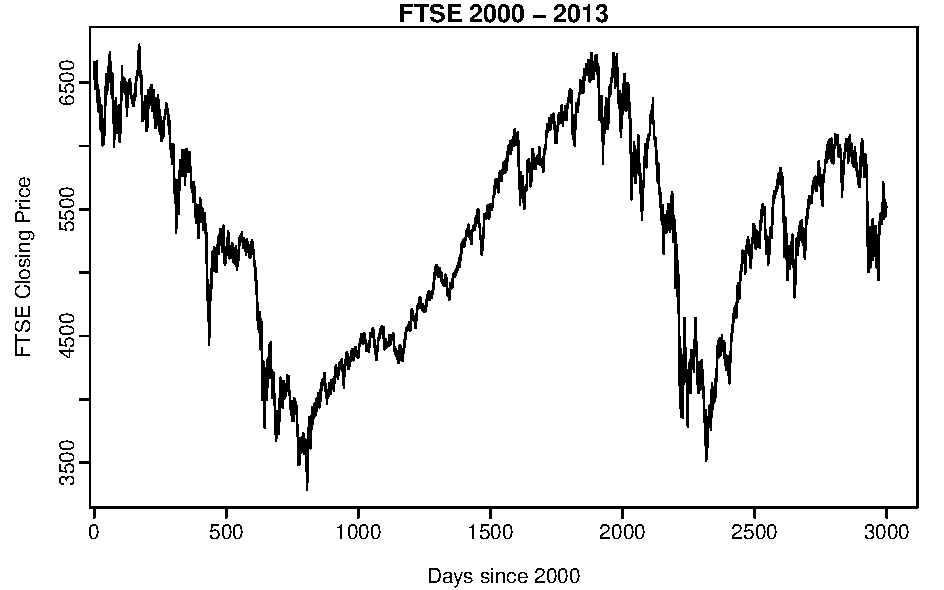
\includegraphics{Figures/chp_ts_ftse_2000-13}
\caption[FTSE 100 index between the years 2000 to 2013]{UK's FTSE 100 index between the years 2000 to 2013.}
\label{fig:chp_ts_ftse_2000_13}
\end{figure}

\subsection{Adjusting for non-uniform variance and non-stationariness}
The variance within the FTSE time series is relatively uniform and thus this data set doesn't need stabilizing with regard to this. If it did, a Box-Cox transformation could be used. However, over this time period the FTSE 100 exhibits marked non-stationariness and requires adjusting accordingly. One such technique to make a data set stationary is differencing. Instead of using the actual observations the differences between two adjacent points are used and this is known as the first difference. If the data set still isn't stationary the difference between consecutive points in the differenced data set can used, this is the difference of the differences and is known as the second difference. Figure \ref{fig:chp_ts_ftse_2000_13_diff} shows the FTSE data set after the first differences have been taken.  The resulting data set is now stationary.

\begin{figure}[tbh]
\centering
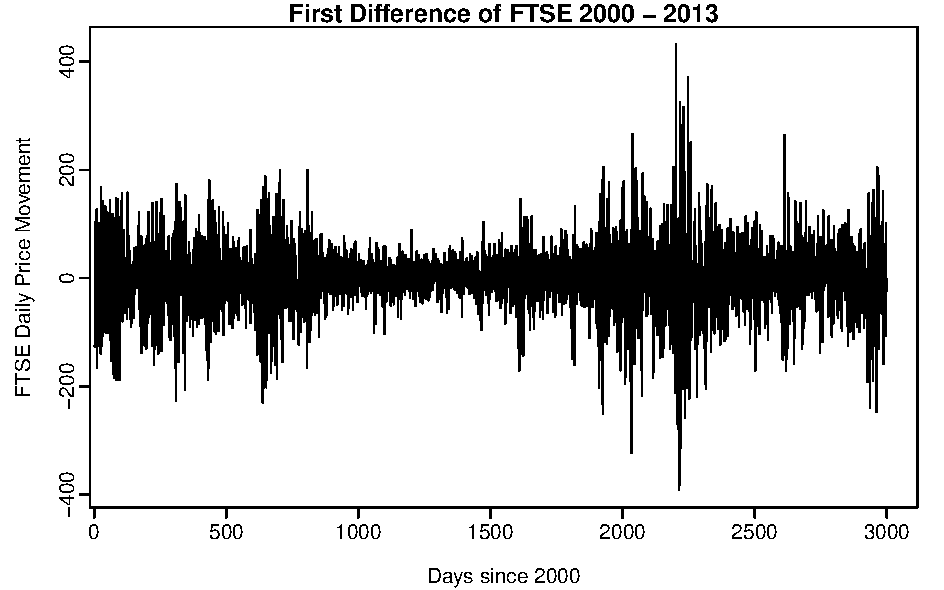
\includegraphics{Figures/chp_ts_ftse_2000-13_diff}
\caption[First difference of FTSE 100 between the years 2000 to 2013]{First difference of FTSE 100 between the years 2000 to 2013.}
\label{fig:chp_ts_ftse_2000_13_diff}
\end{figure}

\subsection{Examine ACF / PACF}
With a stationary data set, the next stage is to investigate the auto-correlation and partial auto-correlation (ACF/PACF) plots in order to help in the model selection process (see section \ref{sec:acf} for details of ACF and PACF). The ACF and PACF for the FTSE data set can be seen in Figures \ref{fig:chp_ts_ftse_2000-13_diff_acf} and \ref{fig:chp_ts_ftse_2000-13_diff_pacf}. 

If ultimately the ARIMA model is of the form ARIMA(p,d,0) or ARIMA(0,d,q) then the ACF and PACF plots are useful in helping to define values for p or q. In the event that both p and q are positive, the ACF and PACF are not helpful in deducing the values for p and q. An ARIMA(p,d,0) model may be appropriate if the ACF and PACF plots of the stationary data exhibit an exponentially decaying pattern in the ACF and a large spike at lag p in PACF plot. Conversely an ARIMA(0,d,q) model may be appropriate if the PACF is decaying exponentially and there is there is a significant spike in the ACF plot at lag q. Considering the ACF and PACF plots in Figures \ref{fig:chp_ts_ftse_2000-13_diff_acf} and \ref{fig:chp_ts_ftse_2000-13_diff_pacf}, neither of the two patterns are observed and thus an ARIMA model where both p and q are positive is likely.

\begin{figure}[tbh]
\centering
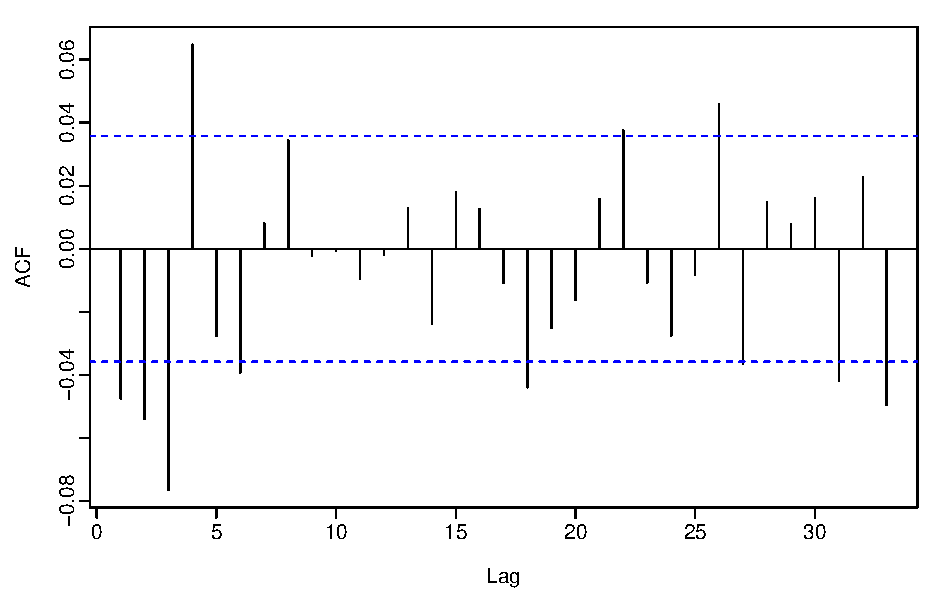
\includegraphics{Figures/chp_ts_ftse_2000-13_diff_acf}
\caption[ACF of FTSE 100 between between the years 2000 to 2013]{Auto-correlation plot of differenced data from FTSE 100 between the years 2000 to 2013.}
\label{fig:chp_ts_ftse_2000-13_diff_acf}
\end{figure}

\begin{figure}[tbh]
\centering
\includegraphics{Figures/chp_ts_ftse_2000-13_diff_pacf}
\caption[PACF of FTSE 100 between between the years 2000 to 2013]{Partial auto-correlation plot of differenced data from FTSE 100 between the years 2000 to 2013.}
\label{fig:chp_ts_ftse_2000-13_diff_pacf}
\end{figure}

%\begin{figure}[tbh]
%\centering
%%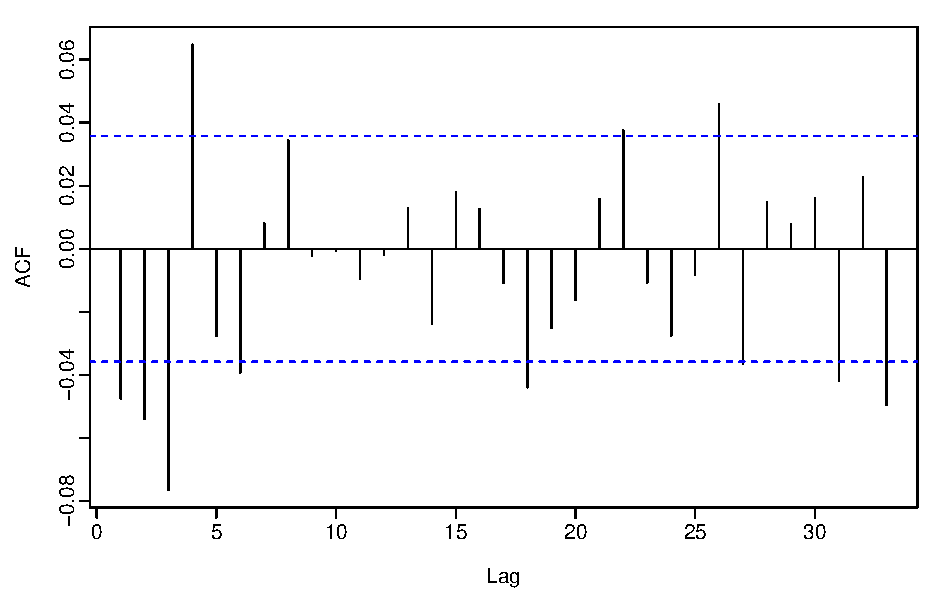
\includegraphics[width=15cm]{Figures/chp_ts_ftse_2000-13_diff_acf}
%\includegraphics[width=14cm, height=12cm]{Figures/chp_ts_ftse_2000-13_diff_acf_tsd}
%\caption[FTSE 2000-13 ACF / PACF.]{Difference, ACF and PACF plots for the FTSE 2000-13.}
%\label{fig:chp_ts_ftse_2000_13_diff_acf_tsd}
%\end{figure}
\textquotesingle\newpage
\subsection{Try the chosen model(s)}
The next step is to try the chosen model along with a few viable alternatives. Akaike’s Information Criterion (AIC) and Bayesian Information Criterion (BIC) are useful for determining the optimum order of an ARIMA model, and are typically used as a measure of how well the model fits the data. AIC can be given by:

\[ AIC = -2 log (L) + 2 (p+q+k+1) \]
where:\\
$ L $ is the likelihood of the data and $ k = 1$ if $c\neq0$ and $ k=0$ if $c \neq 0$, the last term in parentheses is the number of parameters in the model.

For ARIMA models, the corrected AIC can be written as:
\[ AIC_{c} = AIC + \dfrac{2 (p+q+k+1)(p+q+k+2)}{T-p-q-k-2} \]

The Bayesian Information Criterion can be expressed as:
\[ BIC = AIC + log(T)(p+q+k+1) \]

Table \ref{tab:chp_ts:arima_res_r} shows the AIC, AICc and BIC accuracy measures for a selection of ARIMA models applied to the FTSE data set. On all three measures the ARIMA(2,1,3) model has the lowest value.

%label - tab:chp_ts:arima_res_r
% latex table generated in R 3.1.0 by xtable 1.7-3 package
% Thu Aug 21 07:23:05 2014
\begin{table}[ht]
\centering
\caption[AIC, AICc and BIC results from alternative ARIMA models]{AIC, AICc and BIC results from alternative ARIMA models.} 
\label{tab:chp_ts:arima_res_r}
\begin{tabular}{lccc}
  \toprule Model & AIC & AICc & BIC \\ 
  \midrule ARIMA(3,1,1) & 33598.5 & 33598.5 & 33628.5 \\ 
  ARIMA(3,1,2) & 33594.6 & 33594.6 & 33630.6 \\ 
  ARIMA(3,1,3) & 33596.1 & 33596.1 & 33638.1 \\ 
  ARIMA(2,1,1) & 33616.4 & 33616.4 & 33640.4 \\ 
  ARIMA(2,1,2) & 33618.1 & 33618.1 & 33648.1 \\ 
  ARIMA(2,1,3) & 33594.1 & 33594.1 & 33630.1 \\ 
   \bottomrule \end{tabular}
\end{table}


\subsection{Model Residuals}
A so-called residual is the difference between an observation and its forecast. In forecasting a time series, residuals are calculated from a one-step forecast.  A one-step forecast is based on all observations from the start of the series until the previous observation to which the forecast applies to. Thus the number of data points used to calculate the one-step forecast increases as the forecast proceeds through the time series.  An alternative is cross-sectional forecasting which uses all the points in the data set except the observation being predicted.

Knowledge of the residuals from the application of a model is important in establishing the validity of the model. There are two essential and two valuable properties that can be established by inspecting the model residuals. A good method of forecasting will produce a model in which the residuals are uncorrelated and have a zero mean. If a forecasting method doesn't comply with these two properties it can be improved upon. Correlation in residuals means that information is present in them that the model has missed and a non-zero mean is evidence of bias in the forecast. Adjusting for bias is straight forward, the mean value observed in the residuals can simply be added to all forecasts. Looking at Figure \ref{fig:chp_ts_ftse_2000_13_mean_residuals} it can be seen that the mean of the residuals is close to zero and this model doesn't have any bias. Figure \ref{fig:chp_ts_ftse_2000_13_acf_residuals} is the plot of the residuals of the ARIMA model applied to the FTSE data set. The lower order lags are all within the confidence boundaries and is indicative of a good model.

\begin{figure}[!tbh]
\centering
\includegraphics{Figures/chp_ts_ftse_2000-13_mean_residuals}
\caption[FTSE 100 ARIMA model residuals.]{The residuals after applying the ARIMA(2,1,3) model to the FTSE data set.}
\label{fig:chp_ts_ftse_2000_13_mean_residuals}
\end{figure}

\begin{figure}[!tbh]
\centering
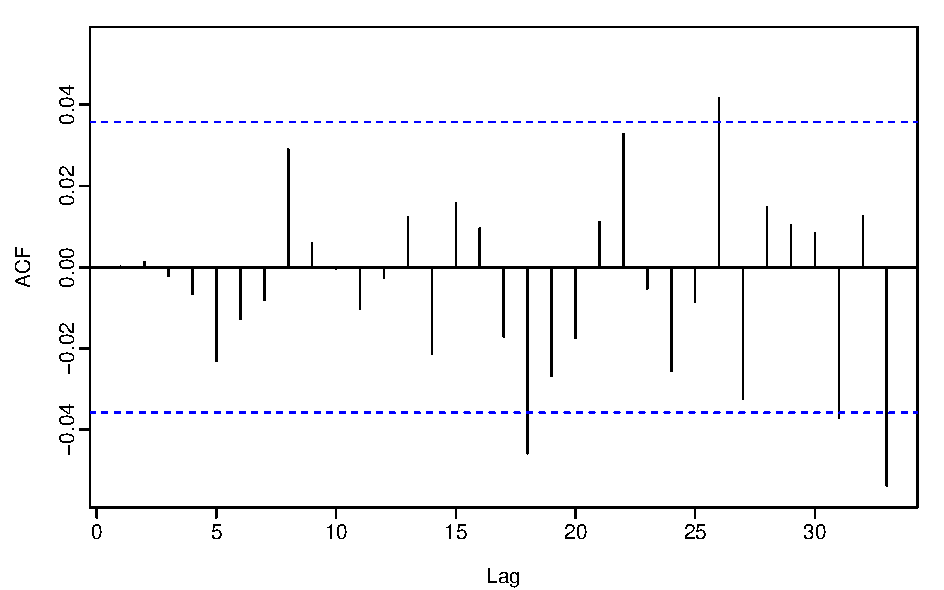
\includegraphics{Figures/chp_ts_ftse_2000-13_acf_residuals}
\caption[ACF plot of the FTSE 100 ARIMA model residuals]{ACF plot of the residuals after applying the ARIMA(2,1,3) model to the FTSE data set.}
\label{fig:chp_ts_ftse_2000_13_acf_residuals}
\end{figure}

Two additional properties of the residuals that are desirable, though not necessary, are constant variance and normal distribution. If these two conditions are met, the calculation of the prediction interval in the forecast step is easier. From Figure \ref{fig:chp_ts_ftse_2000_13_mean_residuals} it can be seen that the residuals have relatively constant variance and from Figure \ref{fig:chp_ts_ftse_2000_13_hist_residuals}, a histogram of the residuals, it can be seen that they are normally distributed.

\begin{figure}[!tbh]
\centering
\includegraphics{Figures/chp_ts_ftse_2000-13_hist_residuals}
\caption[Histogram of the FTSE 100 ARIMA model residuals]{Histogram of the residuals after applying the ARIMA(2,1,3) model to the FTSE data set.}
\label{fig:chp_ts_ftse_2000_13_hist_residuals}
\end{figure}

% Box Ljung test
Consideration of the ACF plots provides evidence for auto-correlation. However a more formal approach is to consider auto-correlation values together as a group as opposed to individually. The Box-Ljung portmanteau test is just one such approach and Table \ref{tab:chp_ts:arima_res_rbox_l} lists the results of the Box-Ljung portmanteau test being applied to the residuals of the ARIMA(2,1,3) model. A large p-value is indicative of white noise and is the desirable situation for a good ARIMA model. Taking all the evidence together the ARIMA(2,1,3) model appears a good option for the FTSE data set.

%label - tab:chp_ts:arima_res_rbox_l
% latex table generated in R 3.1.0 by xtable 1.7-3 package
% Mon Jul 07 19:17:49 2014
\begin{table}[ht]
\centering
\caption[Box Ljung test of FTSE 100 ARIMA model residuals]{Box Ljung test of FTSE 100 ARIMA model residuals.} 
\label{tab:chp_ts:arima_res_rbox_l}
\begin{tabular}{llcc}
  \toprule  & p-value & x-squared & df \\ 
  \midrule ARIMA(2,1,3)                    & 0.2328 & 20 & 24 \\ 
   \bottomrule \end{tabular}
\end{table}


\subsection{Calculate forecast}
Finally, after developing a model that meets the previous criteria a forecast can be generated. Table \ref{tab:chp_ts:ftse_100_fcast} shows the one-step forecast produced when the ARIMA(2,1,3) model developed in the previous section is applied to the FTSE data set.
 
%label - tab:chp_ts:ftse_100_fcast
% latex table generated in R 3.1.0 by xtable 1.7-3 package
% Tue Aug 26 19:01:45 2014
\begin{table}[ht]
\centering
\caption[Forecast for FTSE 100 generated from the ARIMA model]{One-step ahead forecast for FTSE 100 generated from ARIMA(2,1,3) model.} 
\label{tab:chp_ts:ftse_100_fcast}
\begin{tabular}{lccccc}
  \toprule Date & Open & High & Low & Close & Forecast \\ 
  \midrule 20/12/2013 & 6585 & 6617 & 6577 & 6607 & 6560 \\ 
  23/12/2013 & 6607 & 6679 & 6606 & 6679 & 6598 \\ 
  24/12/2013 & 6679 & 6712 & 6672 & 6694 & 6666 \\ 
  27/12/2013 & 6694 & 6754 & 6694 & 6751 & 6692 \\ 
  30/12/2013 & 6751 & 6768 & 6718 & 6731 & 6743 \\ 
  31/12/2013 & 6731 & 6757 & 6731 & 6749 & 6730 \\ 
   \bottomrule \end{tabular}
\end{table}


\section{Automatic Generation of ARIMA Models}
As explained previously the automatic ARIMA modelling algorithm in the R forecast package, auto.arima(), automates steps 3 to 5 in the general steps used in the modelling process as outlined in section \ref{arima_models}. The function uses a variation of the Hyndman and Khandakar algorithm which obtains an ARIMA model by the minimisation of the AICc and combination with unit root tests. KPSS tests are used to establish the number of differences, d, required to get a stationary time series. The p and q values are then obtained by choosing the model that minimises the AICc for the differenced data. 

The results of passing the indice data sets to the auto.arima() function can be seen in Table \ref{tab:chp_ts_arima_models}. For the FTSE data set the automatic procedure selects the ARIMA(2,1,3) as being the most appropriate, which matches the conclusion of the work from the manual model selection process described earlier in section \ref{sec:man_arima}.

%label - tab:chp_ts_arima_models
% latex table generated in R 3.1.0 by xtable 1.7-3 package
% Sat Aug 23 08:35:18 2014
\begin{table}[ht]
\centering
\caption[ARIMA models chosen for the indice data sets]{ARIMA models chosen to forecast future values in the national indice data sets.} 
\label{tab:chp_ts_arima_models}
\begin{tabular}{lc}
  \toprule Market & ARIMA Model \\ 
  \midrule DAX & ARIMA(3,1,3)                    \\ 
  CAC & ARIMA(2,1,3)                    \\ 
  FTSE & ARIMA(2,1,3)                    \\ 
  Dow & ARIMA(1,1,2)                    \\ 
  Nikkei & ARIMA(2,1,3)                    \\ 
  AORD & ARIMA(1,1,0)                    \\ 
   \bottomrule \end{tabular}
\end{table}


\section{Trading the ARIMA Models}
\label{sec:traing:arima:models}
Having developed forecasts based on ARIMA models these can be passed into a trading system. Two ideas are presented here, in the first the previous closing price is compared against the prediction and if it is lower than the forecast a long trade is entered. This first system will be referred to as System 1. In the second algorithm the current forecast is compared with the previous prediction. When the previous forecast value is lower than the current prediction the system trades long. This algorithm will be referred to as System 2.

\subsection{System 1 - Close Price vs Forecast}
Using the ARIMA models listed in Table \ref{tab:chp_ts_arima_models} a series of amended data sets were generated by applying the models to the national indice data sets used throughout this study. The amended data sets contained the original Date, Open, High, Low and Close attributes plus a new one called Forecast, in a similar manner to the data seen in Table  \ref{tab:chp_ts:ftse_100_fcast}. Table \ref{tab:chp_ts:arima1} are results produced from passing the newly generated data sets to the algorithm listed in Appendix \ref{AppendixA} section \ref{appA:ts_1}. This system uses the relative position of the close price and the forecast to determine the direction of the trade. If the forecast is higher than the close a long trade is made and when the prediction is lower than the close price a short trade is made.

%label - tab:chp_ts:arima1
% latex table generated in R 3.1.0 by xtable 1.7-3 package
% Sun Jun 29 08:18:19 2014
\begin{table}[ht]
\centering
\caption[Forecasts generated by the ARIMA models used in the System 1 algorithm]{Forecasts generated by the ARIMA models used in the System 1 algorithm.} 
\label{tab:chp_ts:arima1}
\begin{tabular}{lcccccc}
  \toprule Mkt & LongPL & ShortPL & L Win \% & Av L PL & S Win \% & Av S PL \\ 
  \midrule Dax & -644 & -1881 & 50 & -3 & 41 & -7 \\ 
  CAC & 1555 & 850 & 59 & 6 & 51 & 3 \\ 
  FTSE & 531 & -708 & 53 & 2 & 46 & -2 \\ 
  Dow & 3130 & -1766 & 58 & 14 & 48 & -6 \\ 
  Nikkei & 41 & -1157 & 48 & 0 & 45 & -5 \\ 
  AORD & 679 & -204 & 55 & 3 & 49 & -1 \\ 
   \bottomrule \end{tabular}
\end{table}


\subsection{System 2 - Forecast vs Previous Forecast}
Table \ref{tab:chp_ts:arima2} lists the results from passing the amended indice data sets with the forecasts generated from the auto.arima() function, described in the previous section, to the System 2 algorithm. The R code of this system can be seen in  Appendix \ref{AppendixA} section \ref{appA:ts_2}. System 2 uses the relative values of the forecasts themselves to decide which direction to trade. If the prediction is higher than the previous day's prediction a long trade is initiated and in the opposite circumstances when the previous forecast is higher than the current forecast a short trade is made.

%label - tab:chp_ts:arima2
% latex table generated in R 3.1.0 by xtable 1.7-3 package
% Tue Aug 19 13:19:29 2014
\begin{table}[ht]
\centering
\caption[Results from trading System 2 using the forecasts generated by the ARIMA models]{Results from trading System 2 using the forecasts generated by the ARIMA models.} 
\label{tab:chp_ts:arima2}
\begin{tabular}{lcccccc}
  \toprule Mkt & LongPL & ShortPL & L Win \% & Av L PL & S Win \% & Av S PL \\ 
  \midrule DAX & 733 & -505 & 55 & 3 & 46 & -2 \\ 
  CAC & 545 & -80 & 53 & 2 & 47 & 0 \\ 
  FTSE & 941 & -383 & 54 & 3 & 46 & -2 \\ 
  Dow & 2598 & -2221 & 55 & 9 & 46 & -10 \\ 
  Nikkei & 179 & -916 & 50 & 1 & 47 & -4 \\ 
  AORD & 811 & -117 & 53 & 3 & 46 & 0 \\ 
   \bottomrule \end{tabular}
\end{table}

% ---------------------------------------------------------------
\section{Hybrid ARIMA Models}
\label{sec:arima:chp5}
A hybrid ARIMA model is one in which the moving averages of a stationary data set (possibly a non-stationary data set that has been differenced) are combined with data mining learners other than regression. Possible learners include k nearest neighbour algorithms, artificial neural networks and support vector machines.  RapidMiner, the open source data mining tool is a powerful solution for building hybrid ARIMA models. Figure \ref{fig:chp_ts_rm_arima} shows the RapidMiner process used to generate hybrid ARIMA models. The Validation operator in the model below can hold a variety of learners depending upon the task and data types involved. The various components in Figure \ref{fig:chp_ts_rm_arima} are as follows:

\begin{itemize}
\item Read CSV - reads in the appropriate data set.
\item Select Attribute (1) - selects the attribute that will be processed in the following steps.
\item Rename - renames the attribute selected in Select Attribute (1) to \textquotedblleft attr1" which is then used in the est of the steps. This component is used to make it easy to change the attribute without having to rename all the subsequent steps.
\item Moving Average - calculates a moving average of the time series (see section \ref{sec:chp2_sma} for details.) This provides the q in ARIMA(p,d,q) models.
\item Differentiate - calculates the difference in the time series and provides the d in ARIMA(p,d,q) models.
\item Lag - creates lag variables which are values of the attribute (the attribute itself, the moving average or the difference value) at earlier points in the time series.
\item Select Attribute (2) - selects the attributes that will be passed to the validation block. Attributes regarding today's values are removed because we are building a model to calculate them and don't want to \textquotedblleft peak" at them before the model is built.
\item Set Role - sets an attribute as the label to be predicted.

\end{itemize}

\begin{figure}[!tbh]
\centering
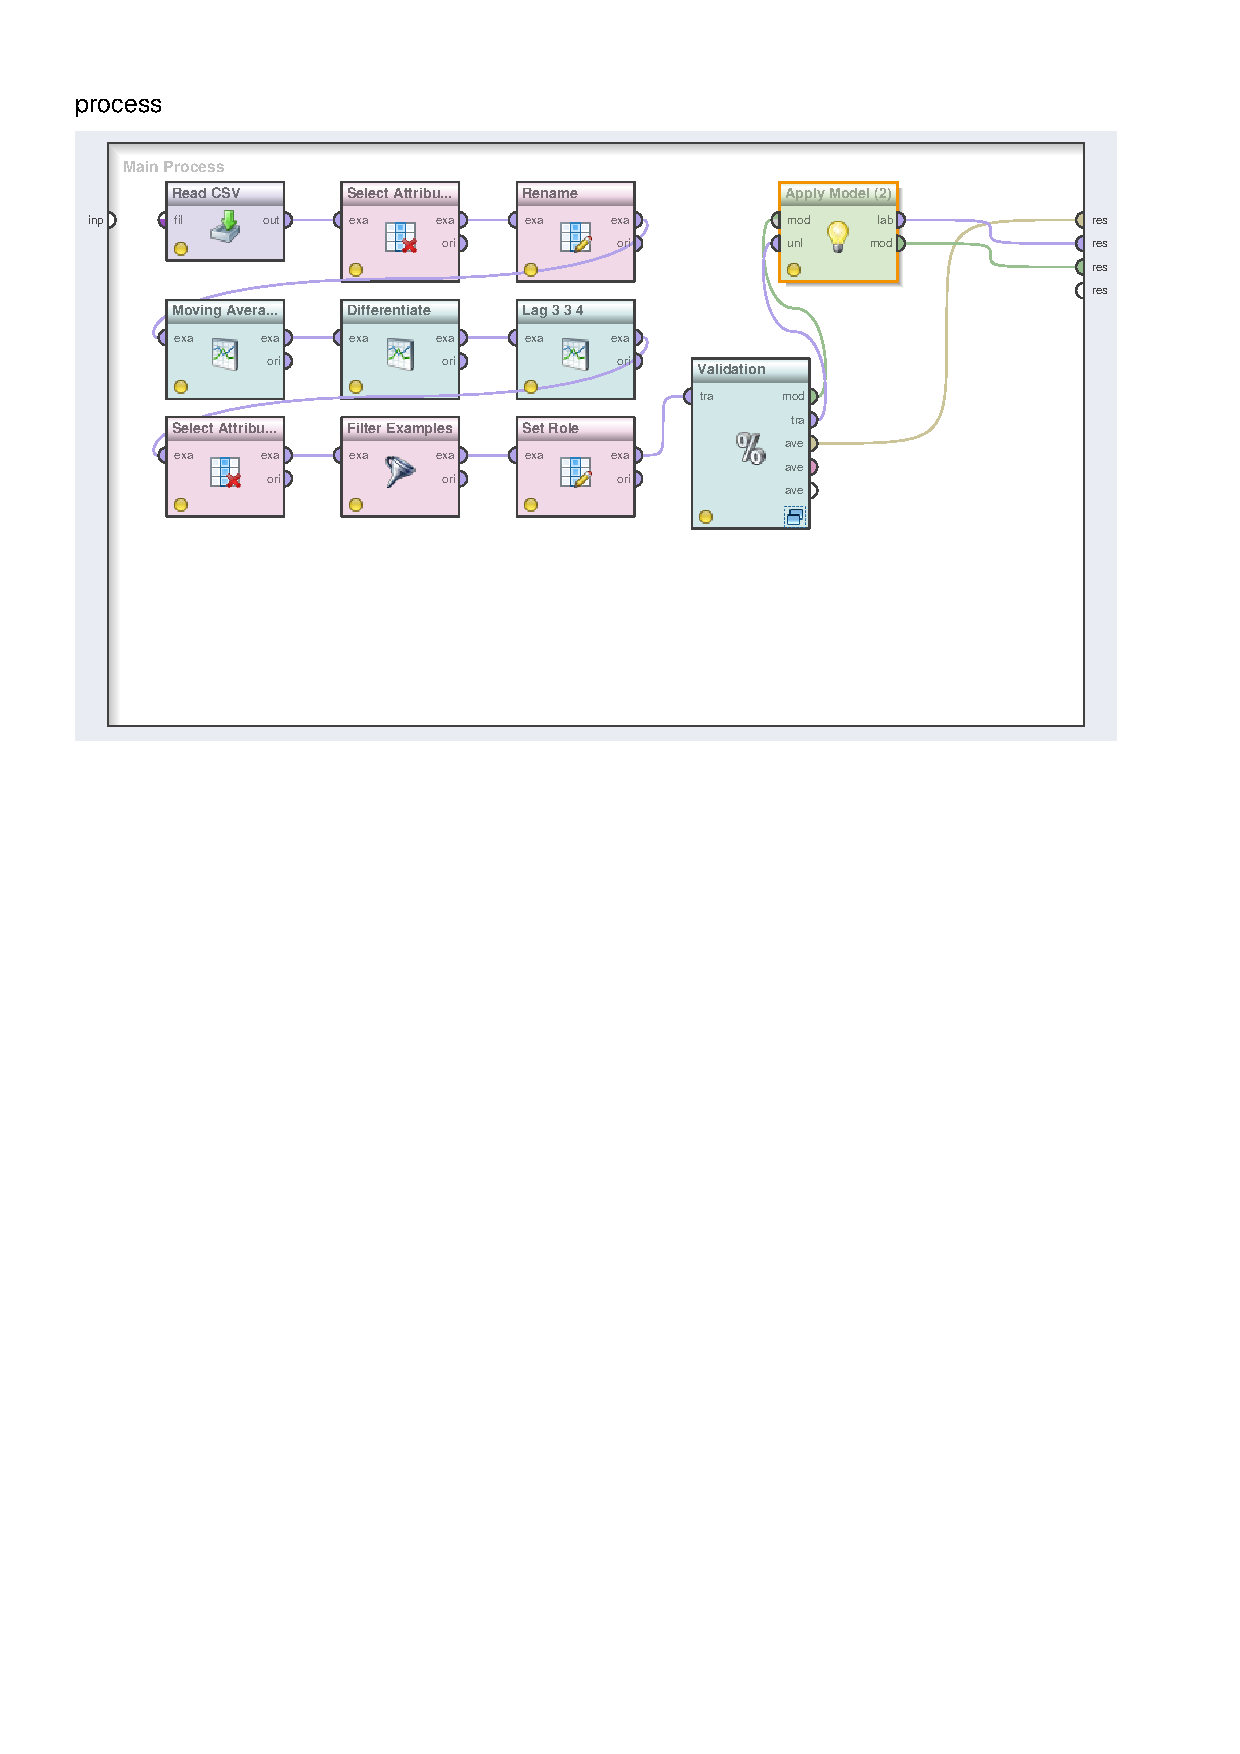
\includegraphics[width=12cm]{../Figures/chp_ts_rm_arima}
\caption[Rapid Miner hybrid ARIMA process]{Rapid Miner hybrid ARIMA process.}
\label{fig:chp_ts_rm_arima}
\end{figure}

Figure \ref{fig:chp_ts_rm_arima_validation} shows the cross-validation operator of the hybrid ARIMA Rapid miner process. This operator can hold alternative learners other than the standard regression operator found in ARIMA models. In the diagram there is an Artificial Neural Network (ANN) operator shown, other options include k-Nearest Neighbour (k-NN) and Support Vector Machine (SVM) operators.

\begin{figure}[h!]
\centering
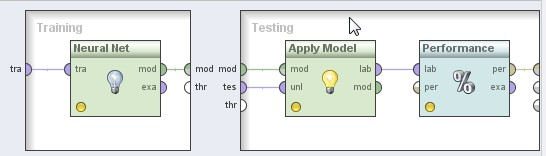
\includegraphics[width=10cm]{../Figures/chp_ts_rm_arima_validation}
\caption[Rapid Miner cross-validation operator]{Rapid Miner cross-validation operator within hybrid ARIMA process.}
\label{fig:chp_ts_rm_arima_validation}
\end{figure}

% ------------------------------------------------------------------------------
\section{Predicting Closing Price}
As mentioned previously ARIMA and hybrid ARIMA models were used to predict either the value of the one-step ahead close price or the binary value of whether the market moved up or down. In this section the ability of hybrid ARIMA models to forecast the future price of financial markets (as opposed to the general direction up or down) is explored.

\subsection{ARIMA/Artificial Neural Networks (ANN)}
An ARIMA/ANN method was used to generate predictions for the closing price of the indice data sets under study. For each data set applying the hybrid model produces a new one-step forecast attribute which can be used in the System 1 and 2 algorithms previously introduced in section \ref{sec:traing:arima:models}. Table \ref{tab:chp_ts:arima_ann_sys1} are the results generated by passing the output of the ARIMA/ANN models to trading System 1 (which compares the previous closing price with the current forecast).

\label{todo:chp5:tab:chp_ts:arima_hybrid_reg}

%label - tab:chp_ts:arima_hybrid_reg
% latex table generated in R 3.1.0 by xtable 1.7-3 package
% Wed Aug 06 18:17:47 2014
\begin{table}[ht]
\centering
\caption[Results from passing closing price predictions from hybrid ARIMA/ANN model to System 1]{Results from passing closing price predictions from hybrid ARIMA/ANN model to System 1.} 
\label{tab:chp_ts:arima_ann_sys1}
\begin{tabular}{lcccccc}
  \toprule Mkt & LongPL & ShortPL & L Win \% & Av L PL & S Win \% & Av S PL \\ 
  \midrule Dax & -5 & -204 & 53 & 0 & 46 & -1 \\ 
  CAC & 355 & 1350 & 56 & 1 & 50 & 2 \\ 
  FTSE & 1692 & 443 & 52 & 2 & 47 & 2 \\ 
  Dow & 2725 & -4100 & 55 & 5 & 44 & -9 \\ 
  Nikkei & 1633 & 2759 & 56 & 6 & 54 & 4 \\ 
  AORD & -898 & -1194 & 52 & -1 & 48 & -4 \\ 
   \bottomrule \end{tabular}
\end{table}


Table \ref{tab:chp_ts:arima_ann_sys2} are the results of passing the output of the ARIMA/ANN models to trading System 2, which compares the value of the current forecast with the previous one.

%label - tab:chp_ts:arima_hybrid_reg
% latex table generated in R 3.1.0 by xtable 1.7-3 package
% Sat Aug 16 11:48:14 2014
\begin{table}[ht]
\centering
\caption[Results from passing closing price predictions from hybrid ARIMA/ANN model to System 2]{Results from passing closing price predictions from hybrid ARIMA/ANN model to System 2.} 
\label{tab:chp_ts:arima_ann_sys2}
\begin{tabular}{lcccccc}
  \toprule Mkt & LongPL & ShortPL & L Win \% & Av L PL & S Win \% & Av S PL \\ 
  \midrule DAX & 3283 & 3110 & 56 & 6 & 49 & 7 \\ 
  CAC & -1832 & -816 & 49 & -3 & 46 & -2 \\ 
  FTSE & 1092 & -182 & 52 & 2 & 48 & 0 \\ 
  Dow & 3829 & -2942 & 54 & 7 & 43 & -7 \\ 
  Nikkei & -4485 & -3229 & 48 & -9 & 50 & -7 \\ 
  AORD & -2783 & -137 & 51 & -5 & 47 & 0 \\ 
   \bottomrule \end{tabular}
\end{table}


\subsection{ARIMA/k-Nearest Neighbour (k-NN)}
An ARIMA/k-NN method was used to generate predictions for the closing price of the indice data sets. Table \ref{tab:chp_ts:pred_close_arima_knn_sys1} shows the results of passing data sets containing forecasts generated with hybrid ARIMA/k-NN to trading System 1.

%label - tab:chp_ts:pred_close_arima_knn_sys1
% latex table generated in R 3.1.0 by xtable 1.7-3 package
% Sun Jun 29 08:18:31 2014
\begin{table}[ht]
\centering
\caption[Results from passing closing price predictions from hybrid ARIMA/k-NN model to System 1]{Results from passing closing price predictions from hybrid ARIMA/k-NN model to System 1.} 
\label{tab:chp_ts:pred_close_arima_knn_sys1}
\begin{tabular}{lcccccc}
  \toprule Mkt & LongPL & ShortPL & L Win \% & Av L PL & S Win \% & Av S PL \\ 
  \midrule Dax & 8270 & 9900 & 56 & 4 & 52 & 6 \\ 
  CAC & 6284 & 12597 & 54 & 3 & 55 & 7 \\ 
  FTSE & 17605 & 17026 & 58 & 9 & 56 & 10 \\ 
  Dow & 30330 & 20549 & 59 & 17 & 53 & 12 \\ 
  Nikkei & 15374 & 33366 & 54 & 9 & 57 & 20 \\ 
  AORD & 7658 & 6638 & 57 & 4 & 53 & 4 \\ 
   \bottomrule \end{tabular}
\end{table}


 Table \ref{tab:chp_ts:pred_close_arima_knn_sys2} shows the results of passing data sets containing forecasts generated with hybrid ARIMA/k-NN to trading System 2.
 
%label - tab:chp_ts:pred_close_arima_knn_sys2
% latex table generated in R 3.1.0 by xtable 1.7-3 package
% Sat Jun 07 08:35:53 2014
\begin{table}[ht]
\centering
\caption[Predicting Close Price - Arima/knn predictions passed to System 2]{Predicting Close Price - Arima/knn predictions passed to System 2} 
\label{tab:chp_ts:pred_close_arima_knn_sys2}
\begin{tabular}{lcccccc}
  \toprule Mkt & LongPL & ShortPL & L Win \% & Av L PL & S Win \% & Av S PL \\ 
  \midrule Dax & 6131 & 7750 & 54 & 3 & 50 & 5 \\ 
  CAC & -567 & 5746 & 50 & 0 & 50 & 3 \\ 
  FTSE & 2571 & 1992 & 52 & 1 & 49 & 1 \\ 
  Dow & 8466 & -1269 & 54 & 4 & 48 & -1 \\ 
  Nikkei & -5066 & 12577 & 49 & -3 & 52 & 8 \\ 
  AORD & 3153 & 2013 & 54 & 2 & 50 & 1 \\ 
   \bottomrule \end{tabular}
\end{table}



% ----------------------------------------------------------------------------------
\section{Predicting Up or Down - Categorical Label}
In this section the ability of hybrid ARIMA models to forecast whether a financial market will rise or fall is investigated. A categorical attribute taking values \textquotedblleft U" and \textquotedblleft D", representing whether the market moved up (\textquotedblleft U") or down (\textquotedblleft D")  was introduced into the indice data sets depending upon which way the market moved that day. Hybrid ARIMA models were used to forecast this categorical label.

\subsection{ARIMA/Artificial Neural Networks (ANN)}
The R code for a trading system using the forecasts from a hybrid model can be seen in Appendix \ref{AppendixA} section \ref{appA:ts_4}. The algorithm simply uses the prediction from the hybrid ARIMA model (\textquotedblleft U" or \textquotedblleft D") to decide whether to trade long or short. Table \ref{tab:chp_ts:pUD_CAT_arima_ann_sys} lists the results from using this hybrid ARIMA/ANN model to make the forecasts.

%Parameters:
%Validation - train/test windows, horizon
%ANN - hidden layers, train cycles, learn rate, momentum 

\label{todo:chp5:tab:chp_ts:pUD_CAT_arima_ann_sys}

%label - tab:chp_ts:pUD_CAT_arima_ann_sys
% latex table generated in R 3.1.0 by xtable 1.7-3 package
% Mon Jun 23 18:28:03 2014
\begin{table}[ht]
\centering
\caption[Results from a trading system using the forecast of categorical label "U/D" from hybrid ARIMA/ANN model]{Results from a trading system using the forecast of categorical label "U/D" from hybrid ARIMA/ANN model.} 
\label{tab:chp_ts:pUD_CAT_arima_ann_sys}
\begin{tabular}{lcccccc}
  \toprule Mkt & LongPL & ShortPL & L Win \% & Av L PL & S Win \% & Av S PL \\ 
  \midrule Dax & 49 & 1714 & 56 & 2 & 48 & 0 \\ 
  CAC & 0 & 6426 & NaN & NaN & 50 & 2 \\ 
  FTSE & 7399 & 6806 & 55 & 5 & 51 & 3 \\ 
  Dow & 12434 & 2711 & 56 & 8 & 49 & 1 \\ 
  Nikkei & -14054 & 3771 & 49 & -4 & 56 & 24 \\ 
  AORD & 3938 & 2978 & 53 & 1 & 59 & 13 \\ 
   \bottomrule \end{tabular}
\end{table}


\subsection{ARIMA/k-Nearest Neighbour (k-NN)}
%Parameters:
%Validation - train/test windows, horizon
%k-NN - k = 15
An Arima/k-NN model was also employed in an attempt to predict the categorical label indicating whether the financial markets would move up or down. The forecasts produced from these hybrid models were also applied to the trading algorithms listed in \ref{AppendixA} section \ref{appA:ts_4}. Table \ref{tab:chp_ts:pUD_CAT_arima_knn_sys} lists the results from this combination.

%label - tab:chp_ts:pUD_CAT_arima_knn_sys
% latex table generated in R 3.1.0 by xtable 1.7-3 package
% Tue Jul 22 20:47:45 2014
\begin{table}[ht]
\centering
\caption[Results from a trading system using the forecast of categorical label "U/D" from hybrid ARIMA/k-NN model]{Results from a trading system using the forecast of categorical label "U/D" from hybrid ARIMA/k-NN model.} 
\label{tab:chp_ts:pUD_CAT_arima_knn_sys}
\begin{tabular}{lcccccc}
  \toprule Mkt & LongPL & ShortPL & L Win \% & Av L PL & S Win \% & Av S PL \\ 
  \midrule Dax & 15692 & 17357 & 61 & 8 & 60 & 12 \\ 
  CAC & 10161 & 16587 & 60 & 6 & 59 & 9 \\ 
  FTSE & 15553 & 14960 & 60 & 8 & 60 & 10 \\ 
  Dow & 30347 & 20624 & 62 & 14 & 60 & 15 \\ 
  Nikkei & 27206 & 45031 & 60 & 18 & 60 & 24 \\ 
  AORD & 9711 & 8751 & 60 & 5 & 59 & 6 \\ 
   \bottomrule \end{tabular}
\end{table}


As the results from Table \ref{tab:chp_ts:pUD_CAT_arima_knn_sys} were good, the algorithm was re-run but this time a stop loss was introduced. A stop loss of 100 points was applied to all the markets and the amended results can be seen in Table \ref{tab:chp_ts:pUD_CAT_arima_knn_sys_SL}. In a similar manner as encountered previously, the use of the stop loss was beneficial for all the markets except the Dow in which case it had a large detrimental affect.

%label - tab:chp_ts:pUD_CAT_arima_knn_sys_SL
% latex table generated in R 3.1.0 by xtable 1.7-3 package
% Tue Aug 26 19:02:10 2014
\begin{table}[ht]
\centering
\caption[Results from a trading system with a stop loss using the forecast of categorical label "U/D" from hybrid ARIMA/k-NN model]{Results from a trading system with a stop loss using the forecast of categorical label "U/D" from hybrid ARIMA/k-NN model.} 
\label{tab:chp_ts:pUD_CAT_arima_knn_sys_SL}
\begin{tabular}{lcccccc}
  \toprule Mkt & LongPL & ShortPL & L Win \% & Av L PL & S Win \% & Av S PL \\ 
  \midrule DAX & -430 & -1444 & 53 & -1 & 47 & -4 \\ 
  CAC & 203 & 1326 & 52 & 0 & 49 & 2 \\ 
  FTSE & 1919 & 526 & 54 & 4 & 50 & 1 \\ 
  Dow & 5475 & -1922 & 51 & 11 & 42 & -4 \\ 
  Nikkei & 4021 & 2804 & 48 & 9 & 49 & 6 \\ 
  AORD & 570 & 3424 & 53 & 1 & 50 & 7 \\ 
   \bottomrule \end{tabular}
\end{table}


%\subsection{ARIMA / Reg}

\subsection{ARIMA/Support Vector Machine (SVN)}
%Parameters:
%Validation - train/test windows, horizon
%k-NN - 

ARIMA was also married with a SVM learner in order to predict the categorical value, \textquotedblleft U" or \textquotedblleft D". Table \ref{tab:chp_ts:pUD_CAT_arima_svm_sys} lists the results of passing forecasts made using this combination to the trading algorithm listed in \ref{AppendixA} section \ref{appA:ts_4}.

%- predicting categorical U / D with ARIMA / ANN. CAC, Oz and 1 other create lopsided predictions ...

%label - tab:chp_ts:pUD_CAT_arima_svm_sys
% latex table generated in R 3.1.0 by xtable 1.7-3 package
% Tue Aug 19 13:19:33 2014
\begin{table}[ht]
\centering
\caption[Results from a trading system using the forecast of categorical label "U/D" from hybrid ARIMA/SVM model]{Results from a trading system using the forecast of categorical label "U/D" from hybrid ARIMA/SVM model.} 
\label{tab:chp_ts:pUD_CAT_arima_svm_sys}
\begin{tabular}{lcccccc}
  \toprule Mkt & LongPL & ShortPL & L Win \% & Av L PL & S Win \% & Av S PL \\ 
  \midrule DAX & -123 & -322 & 53 & 0 & 46 & -1 \\ 
  CAC & -1607 & -612 & 49 & -4 & 47 & -1 \\ 
  FTSE & 2115 & 866 & 54 & 5 & 49 & 1 \\ 
  Dow & 2138 & -4686 & 57 & 10 & 45 & -6 \\ 
  Nikkei & 9 & 1135 & 48 & 0 & 51 & 2 \\ 
  AORD & -2364 & 301 & 53 & -4 & 49 & 1 \\ 
   \bottomrule \end{tabular}
\end{table}


% -------------------------------------------------------------------
%\section{Predicting Up or Down - Continuous Label}
%An alternative to using a categorical variable represented by \textquotedblleft U" or \textquotedblleft D" to indicate if the market rose of fell is to use the numeric range 0 to 1. Here 0 is used to indicate the market fell and 1 to indicate that it increased in value. Thus an additional attribute was introduced into the national indice data sets which took the value of 0 or 1.
%
%\subsection{ARIMA/Artificial Neural Networks (ANN)}
%An ARIMA/ANN model was employed in an attempt to predict the value of 0 or 1, which indicates the directional movement of the market. Table \ref{tab:chp_ts:pUD_01_arima_ann_sys} are the results of passing the indice data sets augmented with the ARIMA/ANN forecasts to the trading algorithm listed in Appendix \ref{AppendixA} section \ref{appA:ts_3a}.
%% EXP algorithm ...
%
%%label - tab:chp_ts:pUD_01_arima_ann_sys
%% latex table generated in R 3.1.0 by xtable 1.7-3 package
% Thu May 29 13:12:22 2014
\begin{table}[ht]
\centering
\caption[Predicting UpDn 01 - Arima/ANN predictions passed to System 2.]{Predicting UpDn 01 - Arima/ANN predictions passed to System 2} 
\label{tab:chp_ts:pUD_01_arima_ann_sys}
\begin{tabular}{lcccccc}
  \toprule Mkt & LongPL & ShortPL & L Win \% & Av L PL & S Win \% & Av S PL \\ 
  \midrule Dax & 316 & 0 & 53 & 0 & NaN & NaN \\ 
   \bottomrule \end{tabular}
\end{table}

%
%\subsection{ARIMA/k-Nearest Neighbour (k-NN)}
%An ARIMA/k-NN model was used to make forecasts for the continuous variable that represents whether the market will move up or down. The output of the model is a value between 0 and 1. The trading algorithm that uses this prediction can be seen in Appendix \ref{AppendixA} section \ref{appA:ts_3} and the results generated in Table \ref{tab:chp_ts:pUD_01_arima_knn_sys}. The trading algorithm looks at the forecast value and trades long if the values are over 0.5 and short if they are below this value.
%
%%label - tab:chp_ts:pUD_01_arima_knn_sys
%% latex table generated in R 3.1.0 by xtable 1.7-3 package
% Sun Jun 29 08:18:37 2014
\begin{table}[ht]
\centering
\caption[Results from a trading system using the forecast of a continous label from a hybrid ARIMA/ANN model]{Results from a trading system using the forecast of a continous label from a hybrid ARIMA/k-NN model.} 
\label{tab:chp_ts:pUD_01_arima_knn_sys}
\begin{tabular}{lcccccc}
  \toprule Mkt & LongPL & ShortPL & L Win \% & Av L PL & S Win \% & Av S PL \\ 
  \midrule Dax & 14122 & 15787 & 64 & 11 & 55 & 7 \\ 
  CAC & 11115 & 17540 & 65 & 10 & 57 & 7 \\ 
  FTSE & 18156 & 17563 & 65 & 14 & 56 & 8 \\ 
  Dow & 28106 & 18383 & 66 & 20 & 55 & 9 \\ 
  Nikkei & 21724 & 39549 & 63 & 25 & 57 & 15 \\ 
  AORD & 9607 & 8647 & 65 & 7 & 56 & 4 \\ 
   \bottomrule \end{tabular}
\end{table}



%\subsection{ARIMA / Regression}
%Using ARIMA with regression to predict 0/1 to represent up and down - See Table \ref{tab:chp_ts:01_arima_reg_sys}
%
%
%%label - tab:chp_ts:01_arima_reg_sys
%% latex table generated in R 3.1.0 by xtable 1.7-3 package
% Fri May 30 21:37:15 2014
\begin{table}[ht]
\centering
\caption[Predicting UpDn 01 - Arima/Reg predictions passed to System 3.]{Predicting UpDn 01 - Arima/Reg predictions passed to System 3} 
\label{tab:chp_ts:01_arima_reg_sys}
\begin{tabular}{lcccccc}
  \toprule Mkt & LongPL & ShortPL & L Win \% & Av L PL & S Win \% & Av S PL \\ 
  \midrule Dax & 749 & 2414 & 53 & 0 & 50 & 4 \\ 
  CAC & 2013 & 8438 & 53 & 1 & 53 & 4 \\ 
  FTSE & 3962 & 3370 & 53 & 2 & 52 & 3 \\ 
  Dow & 13649 & 3925 & 54 & 5 & 52 & 8 \\ 
  Nik & 3633 & 21458 & 52 & 8 & 52 & 7 \\ 
  AORD & 2404 & 1444 & 53 & 1 & 55 & 5 \\ 
   \bottomrule \end{tabular}
\end{table}

